\chapter{Filtre d'Interpolació i Sobremostreig}
\section{Disseny del Filtre de l'Etapa d'Interpolació}
\par Per poder fer el modelat de soroll més endavant i obtenir el rendiment esperat, s'ha implementat una etapa de filtrat i interpolació que aplica un sobremostreig de OSR = 32 dividit en dues etapes. La primera etapa de filtrat es porta a terme en el bloc del filtre FIR, on es sobremostreja l'entrada d'àudio per un OSR = 2. Tot seguit, a l'etapa d'interpolació i filtrat del bloc CIC s'interpola el senyal amb un OSR = 16. En conjunt, els blocs formen el filtre anti-aliasing pre-modulació $\Sigma\Delta$, que millora el rendiment del procés, distribuint el soroll de quantificació inherentment acoblat al senyal d'àudio quantificat i atenua l'amplitud dels harmònics fora de l'ample de banda.    
\par Com s'ha comentat breument a l'apartat 4.6, els filtres CIC són una estructura molt popular en processadors DSP que implementen etapes de sobremostreig o delmat eficients en l'ús de recursos del Hardware. No obstant, per aconseguir una resposta en freqüència amb banda de pas plana i una banda de transició aguda, cal que el bloc CIC vagi precedit d'un filtre compensador. La resposta en freqüència dels filtres CIC ve donada per:
\begin{equation}\label{CIC_magintude_eq}
    \left| H_{CIC}(f) \right| = \left|\frac{1}{RM}\frac{sin(\pi Mf)}{sin(\frac{\pi f}{R})}\right|^N
\end{equation}
On M és el delay diferencial dels blocs Comb, R el factor d'interpolació i N l'ordre del filtre.
\par Com estratègia per aconseguir una banda de pas uniforme i de magnitud 0 dB, es pren la inversa de la magnitud del filtre CIC (equació \ref{CIC_magintude_eq}) per definir la funció de transferència del filtre de compensació. En aplicacions on el producte de R·M $\geq$ 10 i l'ordre del filtre CIC és $\leq$ 7, es pot assumir que la funció de transferència del filtre de compensació es simplifica per la inversa de la funció sinc.\cite{AN455}\cite{Hogenauer1981}
\begin{equation}\label{CIC_compensation_filter_eq}
    \left| H_{Compensation,CIC}(f) \right| = \left|RM\frac{sin(\frac{\pi f}{R})}{sin(\pi Mf)}\right|^N \approx \left| \frac{\pi Mf}{sin(\pi Mf)} \right| ^N = \left|sinc^{-1}(Mf) \right|^N
\end{equation}
\par Per poder calcular els coeficients del filtre de compensació i dimensionar correctament la resposta en freqüència de l'etapa de filtrat en conjunt, s'ha utilitzat el programa MATLAB\textsuperscript{\tiny\textregistered} per la àmplia llibreria disponible per aplicacions en el processament digital de senyals. 
\subsubsection{Filtre de Compensació}
\par Abans de trobar els coeficients que defineixin la resposta en freqüència del filtre, és necessari definir els requisits en rendiment que ha de complir i el context en que s'implementa. A continuació es declaren les especificacions del filtre a implementar:
\begin{table}[H]
    \centering
    \begin{tabular}{ | c | c | }
    \hline
    \centering
     Factor d'interpolació        &  2\\ \hline
     \centering
     Freqüència de pas            &  20 kHz\\ \hline
     \centering
     Freqüència de tall           &  22,05 kHz \\ \hline
     \centering
     Atenuació a la banda de tall &   80 dB\\ \hline
     \centering
     Freqüència de mostreig       &  44,1 kHz \\ \hline
    \end{tabular}
    \caption{Especificacions del filtre de compensació de l'etapa d'Interpolació.}
    \label{taula_filtre_compCIC}
\end{table}
\par Amb les especificacions de la taula \ref{taula_filtre_compCIC} es defineixen els atributs de l'objecte dsp.CICCompensationInterpolator i fent ús de la funció coeffs(), es retorna un vector dels coeficients del sistema. La funció coeffs() retorna un vector de longitud 153 valors que es correspon amb l'ordre del filtre FIR. A la figura \ref{Bode_CompCIC} es pot apreciar el diagrama de Bode del filtre dissenyat.
\begin{figure}[H]
    \centering
    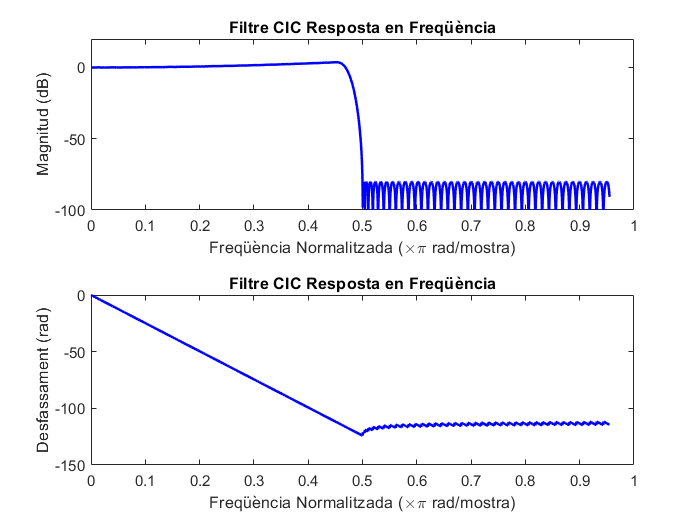
\includegraphics[width=0.5\linewidth]{Images/CIC_CompensationFilter.png}
    \caption{Diagrama de Bode del filtre de compensació de l'etapa d'Interpolació.}
    \label{Bode_CompCIC}
\end{figure}
\subsubsection{Filtre CIC}
A diferència del filtre de compensació, el filtre d'Interpolació CIC no requereix càlculs dels coeficients, degut a que no en té. La resposta en freqüència del filtre en qüestió ve donada per tres paràmetres enters (R, M i N) i la freqüència de mostreig del senyal d'entrada. Modificant el delay diferencial M es pot controlar l'ubicació dels zeros del sistema i en conseqüència la resposta en freqüència. Aquests zeros apareixen en múltiples de $\frac{1}{M}$ i a les regions del voltant d'aquests nuls es produeix l'efecte de l'aliasing. Específicament, aquestes bandes d'àlies són \[(i-f_c) \leq f < (i + f_c)\] per a f $\leq$ $\frac{1}{2}$ i i= 1,2...,[R/2]. Típicament, el paràmetre M sol prendre els valors 1 o 2 permetent una optimització de la implementació del filtre CIC. 
\par Per poder aconseguir la màxima atenuació del soroll en la banda de rebuig o d'aturada, cal modelar l'ordre del filtre fins arribar al valor d'atenuació desitjat. Degut a que la freqüència de Nyquist del senyal passarà a situar-se a R·$f_{Nyquist}$, interessa atenuar el màxim possible la banda de rebuig del senyal original. 
\par Finalment, s'ha trovat que els valors R, M i N del filtre CIC que millor s'adapten als requisits globals de l'etapa de filtrat i sobremostreig són els següents:
\begin{table}[H]
    \centering
    \begin{tabular}{ | c | c | }
    \hline
    \centering
     Factor d'interpolació (R)       &  16\\ \hline
     \centering
     Delay diferencial (M)       &  1\\ \hline
     \centering
     Ordre del filtre CIC (N)        &  5 \\ \hline
    \end{tabular}
    \caption{Especificacions del filtre CIC.}
    \label{taula_filtre_CIC}
\end{table}
\begin{figure}[H]
    \centering
    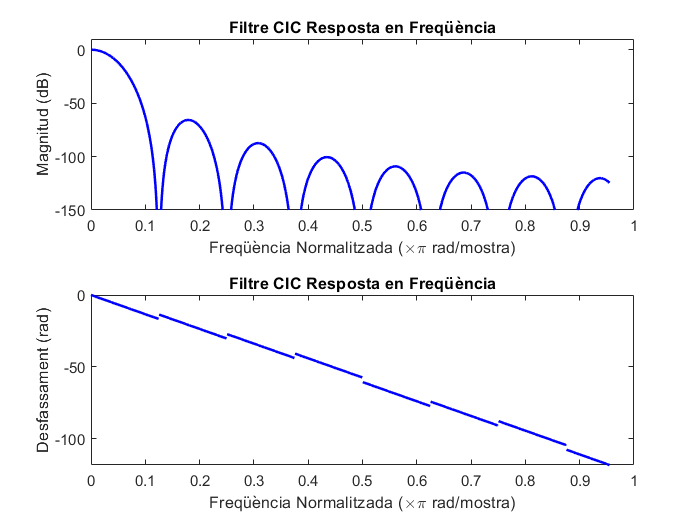
\includegraphics[width=0.5\linewidth]{Images/CIC_Filter.png}
    \caption{Diagrama de Bode del filtre CIC}
    \label{CIC_Bode_fig}
\end{figure}

\subsubsection{Etapa de filtrat i sobremostreig en sèrie}
\par Finalment, situant les dues etapes en sèrie es troba la resposta en freqüència del filtre anti-aliasing. En la figura \ref{fig_BodeEtapaFiltre}, es pot apreciar com la resposta en magnitud a la banda de pas és plana fins la freqüència de tall a $f_c$ = 0,029 $\pi$ rad/mostra, que equival a 20,4 kHz, aproximadament la freqüència de tall de disseny del filtre de compensació (taula \ref{taula_filtre_compCIC}). També es pot apreciar com les imatges ubicades en les proximitats dels zeros del filtre CIC, es veuen atenuades per 50 dB. La resposta en fase decreix linealment, fet que suggereix que el sistema és aproximadament lineal en fase en la banda de pas. La linealitat en la resposta en fase a la banda de pas és rellevant per l'aplicació d'aquest treball degut que en els senyals d'àudio la distorsió de fase provoca anomalies acústiques perceptibles per l'oïda humana. A la taula \ref{taula_mesuresEtapaInterp} estan plasmades les especificacions del etapa d'interpolació del filtre dissenyat.
\begin{figure}[H]
    \centering
    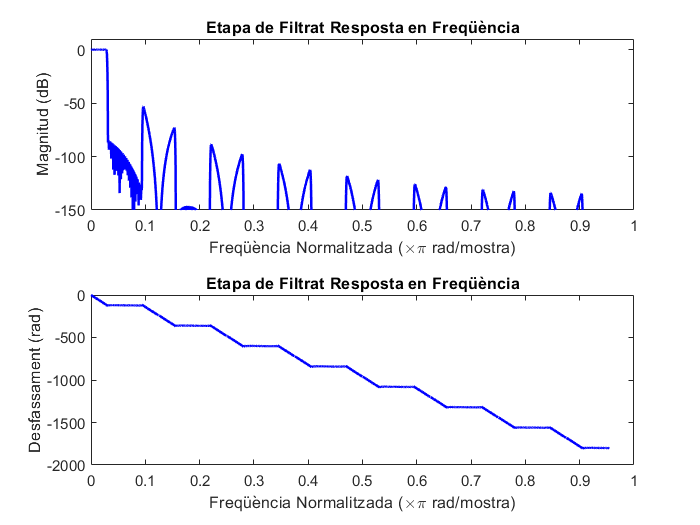
\includegraphics[width=0.5\linewidth]{Images/Etapa_FiltreInterp.png}
    \caption{Diagrama de Bode de l'etapa de filtrat i sobremostreig dissenyada.}
    \label{fig_BodeEtapaFiltre}
\end{figure}
\begin{table}[H]
    \begin{center}
    \begin{tabular}{ | c | c | }
        \hline
        \centering
        Oscil·lació màxima en la banda de pas & 1.49 dB \\ \hline
        \centering
        Freqüència de tall   &  20460 Hz\\ \hline
        \centering
        Atenuació en la banda de tall & -53 dB \\ \hline
    \end{tabular}
    \end{center}
    \caption{Especificacions de l'etapa de filtrat i sobre-mostreig.}
    \label{taula_mesuresEtapaInterp}
\end{table}


\section{Mòdul IP FIR Compiler}
\par Per a la implementació de la primera etapa del filtratge a la FPGA, s'ha utilitzat el mòdul LogiCORE IP FIR Compiler \cite{FIRcompiler}. Aquest bloc permet la sintetització del filtre dissenyat, optimitzant l'utilització dels recursos disponibles a la pròpia FPGA. Per poder implementar el filtre dissenyat en el mòdul en qüestió, cal configurar els paràmetres d'implementació correctament. 
\begin{table}[H]
    \centering
    \begin{tabular}{ | c | c | }
    \hline
    \centering
    \textbf{Nom del Paràmetre}     &  \textbf{Valor}\\ [2ex] \hline
    \centering
    Tipus de Filtre    &    Interpolació \\ \hline
    \centering
    Taxa d'interpolació    &    2 \\ \hline
    \centering
    Format d'Oversampling pel Hardware &    Especificació per freqüència \\ \hline
    \centering
    Freqüència de mostreig d'entrada & 0,0441 MHz \\ \hline
    \centering
    Freqüència de rellotge &    100 MHz \\ \hline
    \centering
    Tipus de coeficients &  Amb signe \\ \hline
    \centering
    Amplada Coeficients & 153 \\ \hline
    \centering
    Tipus de dades d'entrada &  Amb signe \\ \hline
    \centering
    Amplada dades d'entrada &   16 \\ \hline
    \centering
    Mode d'arrodoniment a la sortida & Truncar els LSB \\ \hline
    \centering
    Amplada dades de sortida &  16\\ \hline
    \end{tabular}
    \caption{Configuracions dels paràmetres del mòdul FIR Compiler.}
    \label{taula_configFIR}
\end{table}

\par Inclòs en el mòdul IP hi ha adjunt els arxius de simulació que permeten validar el funcionament del bloc i els respectius pins. A \cite{FIRcompiler} defineixen els pins, destacant-ne els que poden ser d'utilitat per a l'aplicació de la etapa de preacondicionament per la posterior interpolació del filtre CIC:
\begin{itemize}
    \item \textit{aclk}: Entrada del rellotge a la que funcionen els blocs MAC.
    \item \textit{\texttt{s\_axis\_data\_tvalid}}: Entrada que determina en quin instant s’introdueix una mostra.
    \item \textit{\texttt{s\_axis\_data\_tready}}: Sortida que indica que l’estat del filtre és correcte. Cal que aquesta sortida estigui a 1 sempre que el filtre estigui actiu. 
    \item \textit{\texttt{s\_axis\_data\_tdata}}[15:0]: Entrada del vector del valor mostrejat.
    \item \textit{\texttt{m\_axis\_data\_tdata}}[23:0]:  Vector de sortida de la mostra filtrada.
\end{itemize}
\begin{figure}[H]
    \centering
    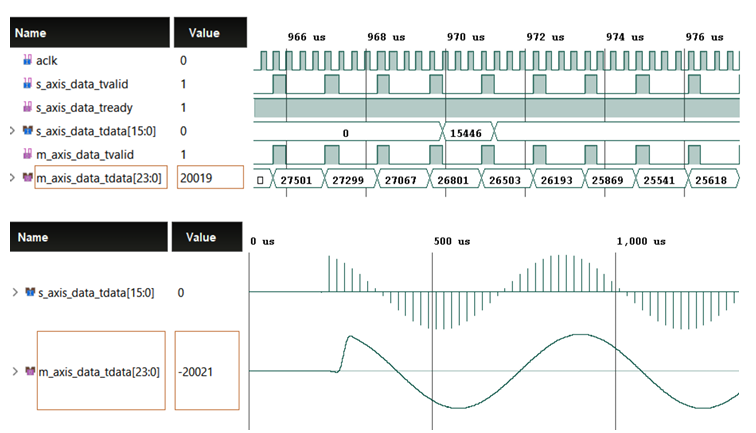
\includegraphics[width=0.6\linewidth]{Images/FIRcompilerTestbench.png}
    \caption{Cronograma del testbench del bloc IP FIR Compiler \cite{TFGAmpClassD}}
    \label{figFIRtestbench}
\end{figure}


\section{Mòdul IP CIC Compiler}
\par Per últim, l'etapa d'Interpolació del CIC s'executa amb el mòdul LogiCORE IP CIC Compiler. Similar al mòdul IP del filtre FIR, aquest permet configurar també els seus paràmetres d'implementació que venen especificats en la taula següent:
\begin{table}[H]
    \centering
    \begin{tabular}{ | c | c | }
    \hline
    \centering
    \textbf{Nom del Paràmetre}     &  \textbf{Valor}\\ [2ex] \hline
    \centering
    Tipus de Filtre    &    Interpolació \\ \hline
    \centering
    Nombre d'etapes    &    5 \\ \hline
    \centering
    Format d'Oversampling pel Hardware &    Especificació per freqüència \\ \hline
    \centering
    Freqüència de mostreig d'entrada & 0,0882 MHz \\ \hline
    \centering
    Freqüència de rellotge &    100 MHz \\ \hline
    \centering
    Amplada dades d'entrada &   16 \\ \hline
    \centering
    Quantització & Truncament \\ \hline
    \centering
    Amplada dades de sortida &  16\\ \hline
    \end{tabular}
    \caption{Configuracions dels paràmetres del mòdul CIC Compiler.}
    \label{taula_configCIC}
\end{table}
\par El mòdul CIC Compiler comparteix el mateix pinatge que el bloc FIR Compiler degut a que ambdós blocs són compatibles amb el bus AXI4 intern de la FPGA. 
\par A la figura \ref{figCICtestbench} es pot apreciar com per cada mostra al pin d'entrada s\textunderscore data\textunderscore t\textunderscore data, es generen 16 mostres a la sortida del bloc.

\begin{figure}[H]
    \centering
    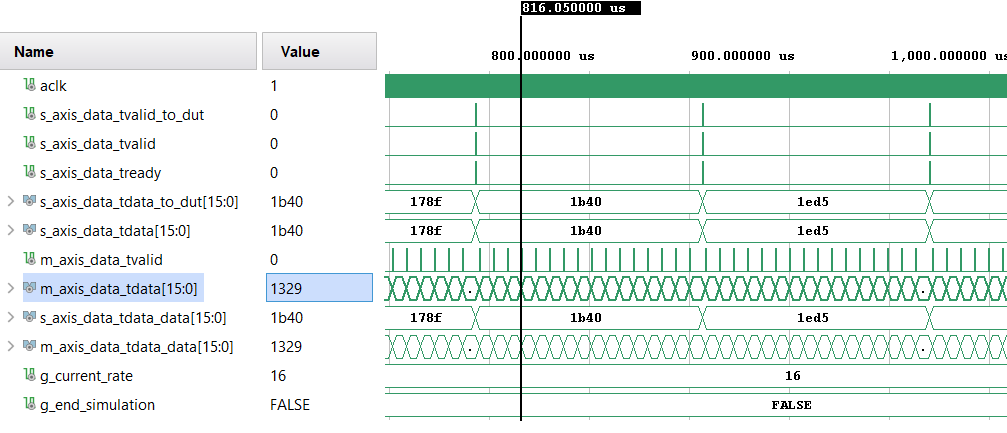
\includegraphics[width=0.6\linewidth]{Images/CICtestbench.png}
    \caption{Cronograma del testbench del bloc IP CIC Compiler.}
    \label{figCICtestbench}
\end{figure}

\section{Implementació a la FPGA}
\par Finalment, la implementació de l'etapa de filtrat i sobremostreig dissenyada en aquest capítol consumeix els recursos detallats a la taula \ref{taularecursosfiltre}. En aquesta taula, destaca l'àmplia utilització de LUTs per part del fir\textunderscore compiler i l'optimització en l'ús dels blocs DSP en els dos mòduls IP.

\begin{table}[H]
    \centering
    \begin{tabular}{ | c | c | c | c | c | c |}
    \hline
    \centering
    \textbf{ID}     &  \textbf{LUTs} & \textbf{Registres}  & \textbf{Slices} & \textbf{Muxes}  & \textbf{DSPs} \\ [2ex] \hline
    \centering
    fir\textunderscore compiler     &  454 & 268  & 79 & 46  & 1 \\ \hline
    \centering
    cic\textunderscore compiler     &  138 & 226  & 56 & 0  & 2 \\ \hline
    \end{tabular}
    \caption{Utilització de recursos de a la FPGA per cada bloc que conforma el filtre antialiasing.}
    \label{taularecursosfiltre}
\end{table}

